\documentclass[a4paper,12pt]{article}

%%% Работа с русским языком
\usepackage{cmap}					% поиск в PDF
\usepackage{mathtext} 				% русские буквы в формулах
\usepackage[T2A]{fontenc}			% кодировка
\usepackage[utf8]{inputenc}			% кодировка исходного текста
\usepackage[english,russian]{babel}	% локализация и переносы

%%% Дополнительная работа с математикой
\usepackage{amsmath,amsfonts,amssymb,amsthm,mathtools} % AMS
\usepackage{icomma} % "Умная" запятая: $0,2$ --- число, $0, 2$ --- перечисление

%% Номера формул
%\mathtoolsset{showonlyrefs=true} % Показывать номера только у тех формул, на которые есть \eqref{} в тексте.
%\usepackage{leqno} % Нумерация формул слева

%% Свои команды
\DeclareMathOperator{\sgn}{\mathop{sgn}}

%% Перенос знаков в формулах (по Львовскому)
\newcommand*{\hm}[1]{#1\nobreak\discretionary{}
{\hbox{$\mathsurround=0pt #1$}}{}}

%%% Работа с картинками
\usepackage{graphicx}  % Для вставки рисунков
\graphicspath{{pictures/}}	%путь к рисункам 
\setlength\fboxsep{3pt} % Отступ рамки \fbox{} от рисунка
\setlength\fboxrule{1pt} % Толщина линий рамки \fbox{}
\usepackage{wrapfig} % Обтекание рисунков текстом

%%% Работа с таблицами
\usepackage{array,tabularx,tabulary,booktabs} % Дополнительная работа с таблицами
\usepackage{longtable}  % Длинные таблицы
\usepackage{multirow} % Слияние строк в таблице

%%% Теоремы
\theoremstyle{plain} % Это стиль по умолчанию, его можно не переопределять.
\newtheorem{theorem}{Теорема}[section]
\newtheorem{proposition}[theorem]{Утверждение}
 
\theoremstyle{definition} % "Определение"
\newtheorem{corollary}{Следствие}[theorem]
\newtheorem{problem}{Задача}[section]
 
\theoremstyle{remark} % "Примечание"
\newtheorem*{nonum}{Решение}

%%% Программирование
\usepackage{etoolbox} % логические операторы

%%% Страница
%\usepackage{extsizes} % Возможность сделать 14-й шрифт
\usepackage{geometry} % Простой способ задавать поля
	\geometry{top=25mm}
	\geometry{bottom=30mm}
	\geometry{left=25mm}
	\geometry{right=25mm}
 %

%%% Способ сделать тоже самое(но красивее:)
%\usepackage[margin=0.8in]{geometry}

 
\usepackage{fancyhdr} % Колонтитулы
 	\pagestyle{fancy}
 	\renewcommand{\headrulewidth}{0mm}  % Толщина линейки, отчеркивающей верхний колонтитул
 	\lfoot{}
 	\rfoot{}
 	\rhead{}
 	\chead{}
 	\lhead{ }
 	% \cfoot{Нижний в центре} % По умолчанию здесь номер страницы

\usepackage{setspace} % Интерлиньяж
%\onehalfspacing % Интерлиньяж 1.5
%\doublespacing % Интерлиньяж 2
%\singlespacing % Интерлиньяж 1

\usepackage{lastpage} % Узнать, сколько всего страниц в документе.

\usepackage{soulutf8} % Модификаторы начертания

\usepackage{hyperref}
\usepackage[usenames,dvipsnames,svgnames,table,rgb]{xcolor}
\hypersetup{				% Гиперссылки
    unicode=true,           % русские буквы в раздела PDF
    pdftitle={Заголовок},   % Заголовок
    pdfauthor={Автор},      % Автор
    pdfsubject={Тема},      % Тема
    pdfcreator={Создатель}, % Создатель
    pdfproducer={Производитель}, % Производитель
    pdfkeywords={keyword1} {key2} {key3}, % Ключевые слова
    colorlinks=true,       	% false: ссылки в рамках; true: цветные ссылки
    linkcolor=red,          % внутренние ссылки
    citecolor=green,        % на библиографию
    filecolor=magenta,      % на файлы
    urlcolor=blue           % на URL
}

%\renewcommand{\familydefault}{\sfdefault} % Начертание шрифта

\usepackage{multicol} % Несколько колонок

% Мои "дополнительные" пакеты
\usepackage{textcase} 
\usepackage{pdfpages}
\usepackage{amsmath}
\usepackage{titlesec}
\usepackage{floatrow}

\usepackage{subfig}

\author{Подкидышев Алексей}
\title{Студент МФТИ ФИВТ - 1ый курс}
\date{\today}

%% Делаем красивый header:
\fancyhead[RO]{\footnotesize{\scshape\nouppercase{~\leftmark}}}
%% Делаем красивый header END

%Делаем большой отступ между section и subsection
\titlespacing*{\section} {0pt}{3.5ex plus 1ex minus .2ex}{2.7ex plus .2ex}
\titlespacing*{\subsection} {0pt}{2.7ex plus 1ex minus .2ex}{1ex plus .2ex}


\begin{document} % конец преамбулы, начало документа

\begin{center}
	\textit{\MakeTextUppercase{федеральное государственное автономное учреждение}}
		
	\vspace{0.5ex}
	
	\textbf{ \\ \MakeTextUppercase{<<Московский Физико-технический институт>>}}
\end{center}
\vspace{13ex}
\begin{flushright}
	\noindent
	{Подкидышев Алексей}
	\\
	\textit{Студенты факультета инноваций\\ и высоких технологий\\(группа 792)}
\end{flushright}
\begin{center}
	\vspace{23ex}
	\line(1,0){430}\\[4ex]
	{\LARGE\textbf{Лабораторная работа 4.2}}
	\vspace{2ex}\\
	\textbf{\large{<<Исследование энергетического спектра $\beta$-частиц при распаде ядер $^{137}$Cs и определение их максимальной энергии при помощи магнитного спектрометра>>}}\\[3ex]
	\line(1,0){430}\\[5ex]
	\vfill
	Долгопрудный 
	
	{\today}
\end{center}

\newpage
\section*{Установка}

\begin{figure}[h!]
	\begin{center}
		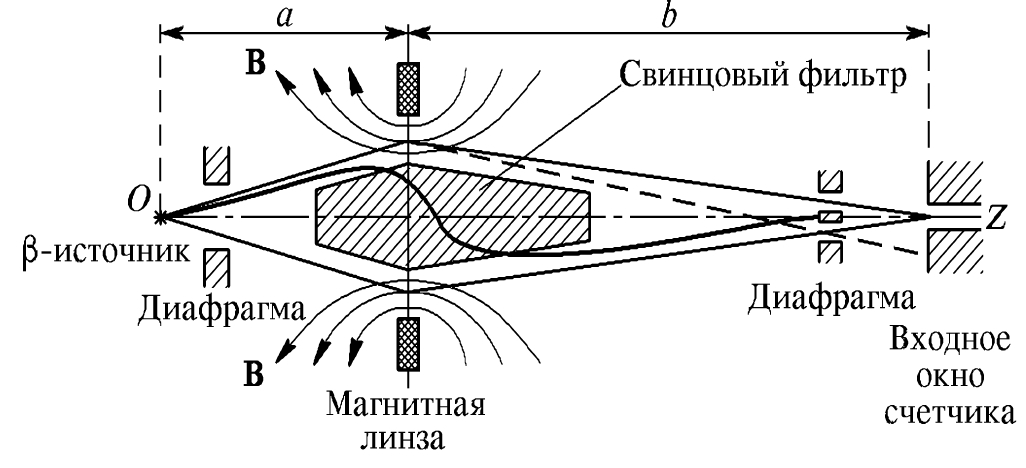
\includegraphics[scale = 0.55]{schem}
		\caption{Схема $\beta$-спектрометра с короткой магнитной линзой}
		\label{ris:schem}
	\end{center}	
\end{figure}

Энергия $\beta$- частиц определяется с помощью $\beta$-спектрометров. В работе используется магнитный спектрометр с "короткой линзой". Для заряженных частиц тонкая катушка эквивалентна линзе и её фокусное расстояние зависит от импульса электронов и от индукции магнитного поля (т.е. от силы тока, протекающего через катушку):
\begin{equation}
\frac{1}{f} \simeq \frac{I^2}{p_e^2}
\end{equation}

Следовательно фокусируются только электроны с определённым импульсом и отсюда можно получить распределение по импульсам, определив коэффициент пропорциональности из опыта по какому-нибудь известному значению импульса (значению известной конверсионной линии): 
\begin{equation}
p_e = kI
\end{equation}


\section*{Теоретические сведения}
	Бета-распад это самопроизвольное преваращение ядер, при котором их массовове число не изменяется, а заряд изменяется на единицу. Выделяюющаяся при одном акте $\beta$-распада энергия варьируется от 18 кэВ ($^{3}_{1}H$) до 13,4 МэВ ($^{12}_{15}B$). В~данной работе мы будем иметь дело с электронным распадом:\\
	\begin{equation}
	_{Z}^{A}X \rightarrow ^{A}_{Z+1}X + e^{-} + \widetilde{\nu},
	\end{equation}
	
	Освобождающаяся в результате распада энергия делится между дочерним ядром, электроном и антинейтрино. При этом доля энергии, уносимая ядром крайне мала, так что можно считать, что вся энергия делится между антинейтрино и электроном. Поэтому электроны могут иметь любую энергию от нулевой до некоторой макимальной энергии, высвобождаемой при распаде.
	
	Вероятность $d\omega$ того, что электрон вылетит с имульсом $d^3\mathbf{p}$, а нейтрино с импульсом $d^3\mathbf{k}$ пропорциональна произведению этих дифференциалов, но мы должны учесть также закон сохранения энергии:
	\begin{equation}
	E_e - E - ck = 0,
	\label{zse}
	\end{equation}
	где $E_e$ -- максимальная энергия электрона, $E$ -- энергия электрона. Релятивистская связь энергии электрона с импульсом:
	\begin{equation}
	E = c\sqrt{p^2 + m^2c^2} -mc^2
	\end{equation}
	
	Тогда, вводя $\delta$-функцию для учёта условия (\ref{zse}), вероятность $d\omega$ принимает вид:
	\begin{equation}
	d\omega = D\delta(E_e-E-ck)d^3\mathbf{p}d^3\mathbf{k} = D\delta(E_e-E-ck)p^2d pk^2d kd\Omega_ed\Omega_{\widetilde{\nu}},
	\end{equation}
	где D -- некоторый коэффициент пропорциональности, который можно считать с хорошей точностью константой. В этом случае можно проинтегрировать по всем углам и по абсолютному значению импульса антинейтрино. В этом случае $\delta$-функция исчезнет, а $ck$ всюду заменится на $E_e-E$. После умножения на полное число распадов $N_0$ получим число электронов $dN$, вылетающих из ядра с модулем импульса из промежутка $[p;p+dp]$:
	\begin{equation}
	d N = \frac{16\pi^2N_0}{c^2} D p^2\left(E_e-E\right)^2d p
	\end{equation}
	
	Выразив из (\ref{zse}) $dE$, получим распределение электронов по энергиям:
	\begin{equation}
	\dfrac{dN}{dE} = N_0B\sqrt{E(E+2mc^2)}(E_e - E)^2(E + mc^2), \qquad B = \dfrac{16\pi^2D }{c^4},
	\end{equation}
	
	В нерелятивистском случае выражение упрощается и принимает вид:
	\begin{equation}
	\frac{d N}{d E} \simeq \sqrt{E}(E_e - E)^2
	\end{equation} 
	
	Вид полученного распределения с учётом конверсионных электронов: 
	\begin{figure}[h!]
		\centering
		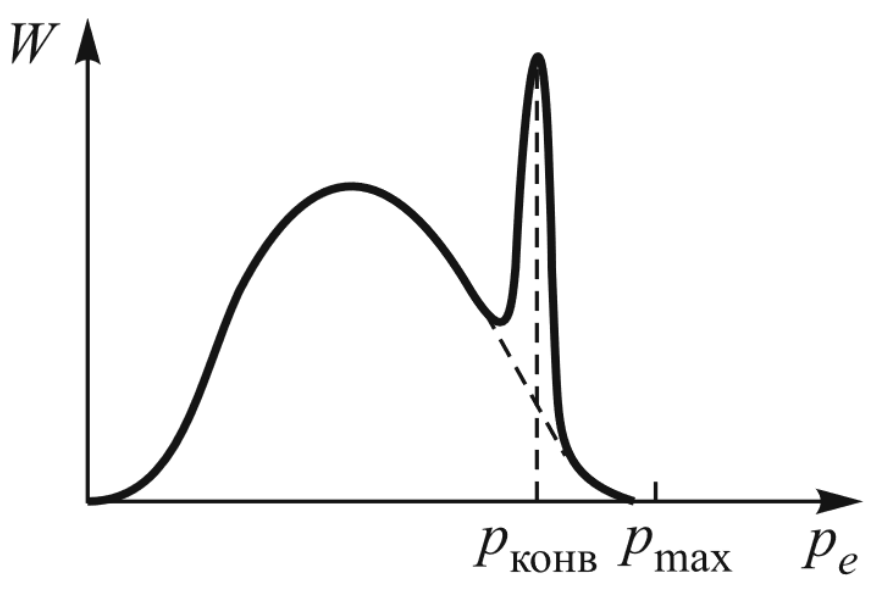
\includegraphics[width=0.38\linewidth]{pic1}
		\caption{Форма спектра $\beta$-частиц при разрешенных переходах}
	\end{figure}

	Упомянутые выше конверсионные электроны возникают вследствие возбуждённого состояния дочернего ядра (нередко возникающего после $\beta$-распада). Образовавшийся избыток энергии ядро сбрасывает в виде $\gamma$-кванта, либо передавая её электрону на внутренних оболочках. Полученные конверсионные электроны имеют строго определённую энергию. Чаще всего  конверсия происходит на K или L оболочках.

\section*{Экспериментальная часть}

Создав в полости спектрометра вакуум, снимем зависимость количества регистрируемых частиц $N$ от силы тока в линзе $I$. \\

\textit{Фоновое излучение}: $1,300~с^{-1}$\\

\textit{Время измерения}: $80~с$\\ 

\begin{figure}[h!]
	\centering
	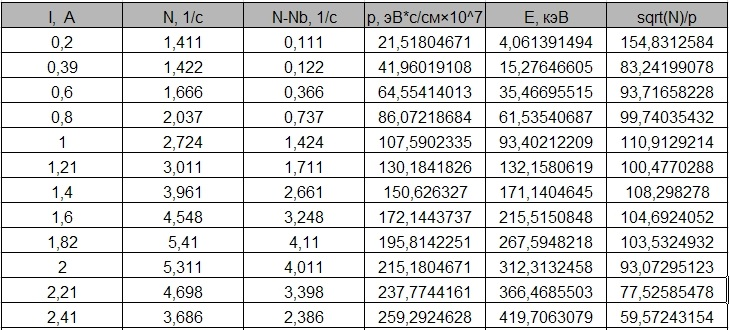
\includegraphics[width=0.9\linewidth]{tbl1}
\end{figure}

\begin{figure}[h!]
	\centering
	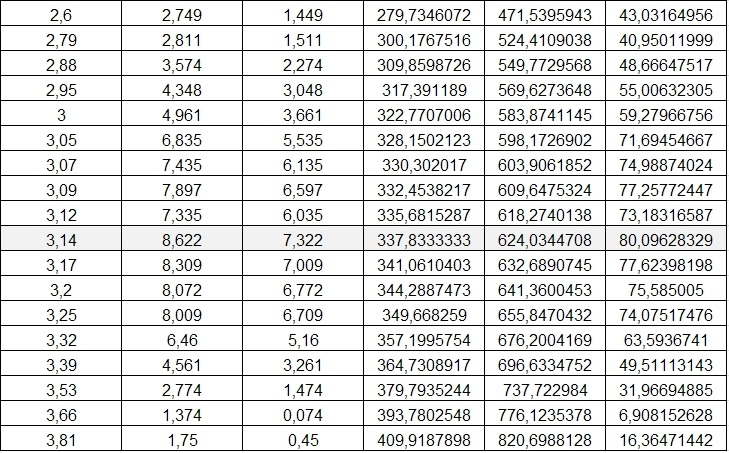
\includegraphics[width=0.9\linewidth]{tbl2}
\end{figure}

Построим график Ферми-Кюри и его часть на линейном участке (для определения максимальной энергии электронов, как пересечение графика с осью $E$):\\

\begin{figure}[h!]
	\centering
	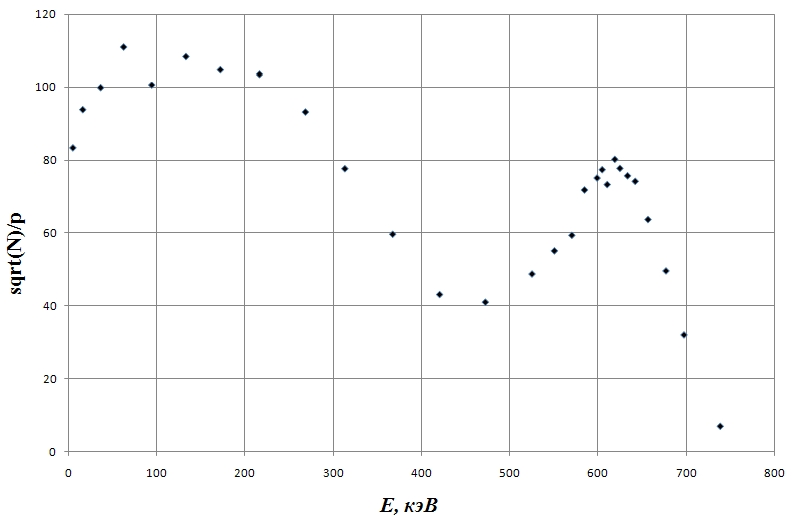
\includegraphics[width=0.9\linewidth]{gr1}
\end{figure}

\begin{figure}[h!]
	\centering
	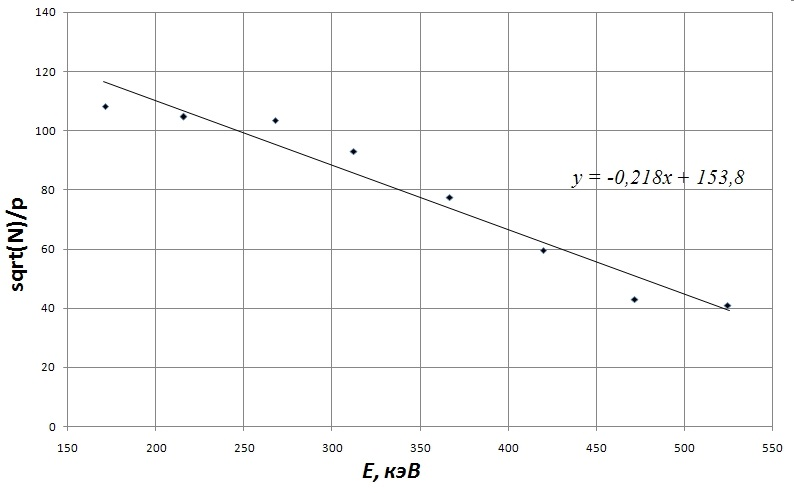
\includegraphics[width=0.9\linewidth]{gr2}
\end{figure}

\newpage
$$E_e = (705 \pm 150)~\text{кэВ}$$

\vspace{-10pt}
\section*{Вывод:}   В проделанной работе было исследовано явление $\beta$-распада $^{137}Cs$. Выявлен <<полудискретный>> характер спектра: непрерывная часть обеспечивается за счет рождения электрона и антинейтрино, дискретный пик --- рождение конверсионных электронов. Непрерывность спектра доказывает существование антинейтрино и его рождение в процессе $\beta^-$ распада. Также было показано существование конверсионных электронов --- электронов, испускаемых в результате перехода ядра на более низкий энергетический уровень. Их энергетический спектр является уже дискретным, т.к. их энергия строго привязана к энергетическим уровням ядра.


\end{document}